\documentclass[../../main.tex]{subfiles}

\begin{document}

%\newcommand{\statement}[1]{\textrm{\enquote{\textbf{#1}}}}
\newcommand{\statement}[1]{\textrm{\fontencoding{T1}\fontsize{10}{12}\fontfamily{put}\itshape\selectfont#1}}

%\newcommand{\centralizedImage}[3]{
%   \ifthenelse{\equal{#3}{}}
%   {
%   \begin{minipage}[c][][c]{#2cm}
%       \includegraphics[height=1cm]{#1}
%   \end{minipage}
%   }
%   {
%   \begin{minipage}[c][][c]{#2cm}
%    \begin{tikzpicture}
%       \node at (0,0) {\includegraphics[height=1cm]{#1}};
%       \draw[line width=2mm,red,opacity=0.6] (-.5,-.5) -- (.5,.5);
%       \draw[line width=2mm,red,opacity=0.6] (.5,-.5) -- (-.5,.5);
%    \end{tikzpicture}
%   \end{minipage}
%   }
%}
\newcommand{\statementIcon}[3]{
    \begin{tikzpicture}[onbase]
        \node at (0,0) {\includegraphics[height=1cm]{#1}};
        \ifthenelse{\equal{#3}{}}{}{
            \draw[line width=2mm,red,opacity=0.6] (-.5,-.5) -- (.5,.5);
            \draw[line width=2mm,red,opacity=0.6] (.5,-.5) -- (-.5,.5);
        }
    \end{tikzpicture}
}
\def\poisonIcn{\statementIcon{images/poison.png}{0.86}{}}
\def\superPwrIcn{\statementIcon{images/super_power.png}{0.86}{}}
\def\superPwrIcnVarI{\statementIcon{images/super_power_index1.png}{0.86}{}}
\def\superPwrIcnVarII{\statementIcon{images/super_power_index2.png}{0.86}{}}
\def\drinkIcn{\statementIcon{images/trinken_TEMP.png}{0.86}{}}
\def\burgerIcn{\statementIcon{images/burger.png}{1.53}{}}
\def\saladIcn{\statementIcon{images/salat.png}{1.39}{}}
\def\friesIcn{\statementIcon{images/pommes.png}{0.86}{}}

\todo{einheitlich bold, anführungszeichen}
\todo{irgendwo erwähnen, dass man streng genommen auch um Negation klammern müsste ( $\lnot (A \implies B)$, vs $(\lnot A) \implies B$), wir lassen das aber aus platzgründen weil, wir nicht am stärksten binden soll. Im letzten beispiel wird negations geklammert}

In diesem Abschnitt möchten wir den Aufbau von Aussagen genauer untersuchen. Dabei lernen wir verschiedene Typen von Aussagen kennen und lernen, in welchen Situationen man diese anwenden kann. Außerdem wird gezeigt, wie man Aussagen formalisieren kann. Etwas zu formalisieren, bedeutet so viel wie etwas mathematisch aufzuschreiben.

Wir stellen zunächst fest, dass wir mehrere Aussagen zu einer neuen Aussage kombinieren können, indem wir diese durch Bindewörter wie dem \statement{und} verknüpfen.
\begin{example}{}
    \parpic[r]{
        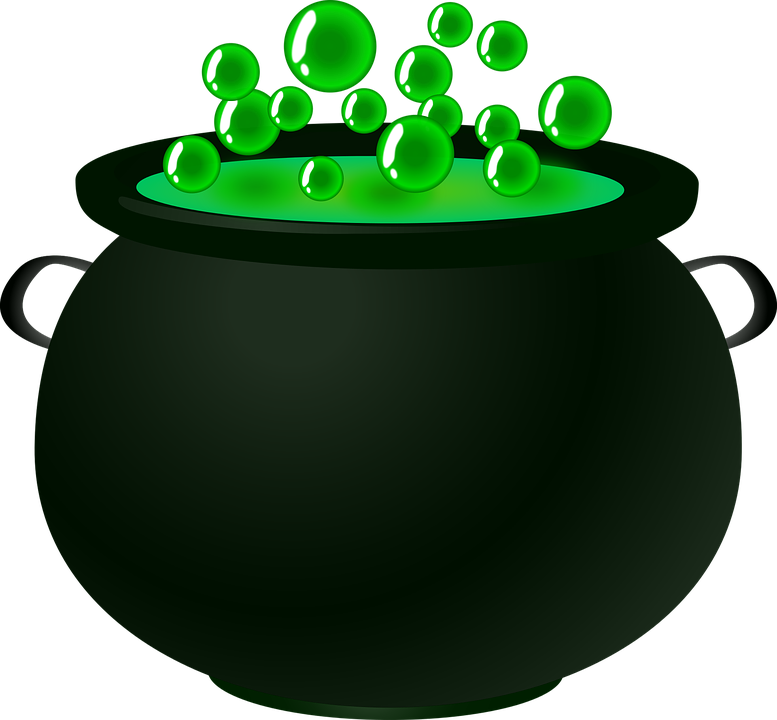
\includegraphics[width=0.2\textwidth]{images/Zaubertrank.png}
    }
    Die zwei Sätze
    \statement{Der Trank ist giftig} und \statement{Ich trinke den Zaubertrank}
    sind beides Aussagen. Wir können nun aus diesen Aussagen eine neue Aussage basteln. Wir verknüpfen dazu die beiden Aussagen mit einem \statement{und} zu einer neuen Aussage. Die resultierende Aussage lautet wie folgt: \statement{Der Trank ist giftig und ich trinke den Zaubertrank}.
\end{example}

Aussagen lassen sich aber auch durch andere Wörter, abgesehen von \statement{und} verknüpfen. Dazu gleich mehr. Solche Wörter, die Aussagen miteinander zu einer neuen Aussagen verknüpfen, nennen wir \textbf{Konnektoren}. Das kommt aus dem Englischen von \enquote{to connect}, was verbinden heißt. Das Wort \statement{und} ist also ein Konnektor.

\begin{definition}{}
Ein Wort oder eine Kombination von mehreren Wörtern, die Aussagen miteinander zu einer neuen Aussage verknüpfen, nennt man einen Konnektor.
\end{definition}

\begin{lemma}{}
Das Wort \statement{und} ist ein Konnektor.
\end{lemma}

Jetzt wird ein neuer Typ von Aussagen vorgestellt.
\begin{example}{}
Die Aussage \statement{Der Zaubertrank ist giftig und ich trinke ihn} besteht aus zwei kleineren Aussagen, nämlich:
\begin{enumerate}
    \item \statement{Der Zaubertrank ist giftig}
    \item \statement{Ich trinke den Zaubertrank}
\end{enumerate}
Wobei die zweite, kleinere Aussage nicht wortwörtlich vorkommt, aber sinngemäß.
Diese beiden kleineren Aussagen nennen wir \textbf{Unteraussagen} der größeren Aussage.
\end{example}

\begin{definition}{}
Aussagen, die Teil einer Aussage sind, nennen wir \textbf{Unteraussagen}.
\end{definition}


Bevor wir jetzt weitere Typen von Aussagen und Konnektoren vorstellen, wollen wir uns zunächst das Leben einfacher machen.
In der Mathematik möchte man, wenn möglich, Schreibarbeit sparen. Wir zeigen daher jetzt, wie man Aussagen etwas kürzer und prägnanter notieren kann.

\begin{example}{}
Wir wollen die Aussage aus letztem Beispiel \statement{Der Zaubertrank ist giftig und ich trinke ihn} kürzer notieren. Um das zu erreichen, denken wir uns Symbole für jede der zwei Unteraussagen aus. Anstatt den Unteraussagen schreiben wir dann nur noch die ausgedachten Symbole, welche dann stellvertretend für die Unteraussagen stehen. 
Wir wählen folgende Symbole für die Unteraussagen:
 \[\underbrace{\statement{Der Zaubertrank ist giftig}}_{\poisonIcn}\statement{~und~}\underbrace{\statement{ich trinke ihn}}_{\drinkIcn}\]
 Wenn wir nun diese Symbole anstelle von den ausformulierten Unteraussagen schreiben, dann erhalten wir eine deutlich verkürzte Schreibweise für unsere Aussage. Die verkürzte Schreibweise sieht dann wie folgt aus:
 \begin{center}
        \poisonIcn
        \statement{und}
        \drinkIcn
  \end{center}
\end{example}

Um Schreibarbeit zu sparen, bietet es sich an, Unteraussagen einer Aussage durch Symbole oder Bilder zu ersetzen, die dann stellvertretend für die Unteraussage stehen. So müssen wir nicht immer die gesamte Unteraussage aufschreiben, sondern wir müssen dann nur das Bild bzw. das Symbol zeichnen. Das werden wir von nun an, sofern möglich, immer machen.

Wir haben bereits gesehen, dass wir mit Konnektoren, Aussagen miteinander verknüpfen können. Dabei haben wir bereits den Konnektor \statement{und} kennengelernt.
Neben diesem Konnektor gibt es aber auch noch weitere. Diese werden jetzt vorgestellt.

\begin{example}{}
    Ein Zauberer überreicht dir 2 Zaubertränke. Beide Zaubertränke sind entweder giftig oder verleihen Superkräfte. Der Zauberer garantiert dir, dass aber mindestens einer der beiden Tränke Superkräfte verleiht. Es könnte also auch passieren, dass beide Tränke Superkräfte verleihen.
    
    Diesen Sachverhalt wollen wir als Aussage formulieren. Wir führen vorher Abkürzungen ein, um uns wieder Schreibarbeit abzunehmen. Folgende Tabelle zeigt die Abkürzungen:
    
    \begin{tabular}{@{}c@{:~}l@{}}
         \superPwrIcnVarI & \statement{Der 1. Trank verleiht Superkräfte}\\
         \superPwrIcnVarII & \statement{Der 2. Trank verleiht Superkräfte}
    \end{tabular}
    
    Mit diesen Abkürzungen können wir nun den Sachverhalt, nämlich, dass mindestens einer der Tränke Superkräfte verleiht, als Aussage formulieren.
    \[\superPwrIcnVarI \statement{ oder } \superPwrIcnVarII\]
    Mit dem Konnektor \statement{oder} kann man also ausdrücken, dass mindestens eine von zwei Aussagen zutrifft. Es kann also durchaus auch sein, dass beide Aussagen zutreffen. In diesem Beispiel könnten nämlich auch beide Tränke Superkräfte verleihen.
\end{example}

Haben wir zwei Aussagen gegeben und möchten wir in einer neuen Aussage formulieren, dass wir auf mindestens eine der zwei Aussagen mit \enquote{Ja, das ist wahr} antworten können, dann können wir das mit der Aussage \statement{[Erste Aussage] oder [Zweite Aussage]} ausdrücken. Wir verbinden also einfach die beiden Aussagen mit dem Konnektor \statement{oder}.

\begin{lemma}{}
    Das Wort \statement{oder} ist ein Konnektor.
\end{lemma}

Jetzt wird noch eine andere Art vorgestellt, wie man Aussagen verknüpfen kann.

\begin{example}{}
    Du hast wieder einen Zaubertrank vor dir. Entweder der Zaubertrank ist giftig oder er verleiht Superkräfte. Du hättest gerne Superkräfte. Deswegen würdest du den Trank trinken, wenn du wüsstest, dass es sich um den Superkräfte-Zaubertrank handelt. Wir wollen dein Verhalten wieder als Aussage formulieren. Dazu verwenden wir folgende Abkürzungen:
    
    \begin{tabular}{@{}c@{:~}l@{}}
         \superPwrIcn & \statement{Der Trank verleiht Superkräfte}\\
         \drinkIcn & \statement{Ich trinke den Trank}
    \end{tabular}
    
    Wir können dein Verhalten nun durch folgende Aussage beschreiben:
    \[\statement{Wenn }\superPwrIcn\statement{ dann }\drinkIcn\]
    Diese Aussage ist eine sogenannte Implikation. Verknüpft man zwei Aussagen mit den Konnektoren \statement{wenn, dann}, dann erhält man eine Implikation. Man nennt die Aussage auf die sich das \statement{wenn} bezieht, die Bedingung. Hier ist das \statement{Der Zaubertrank verleiht Superkräfte}. Die Aussage auf die sich \statement{dann} bezieht, nennt sich die Konsequenz aus der Bedingung. Hier ist das \statement{Ich trinke den Zaubertrank}.
\end{example}

Wir fassen die Erkenntnisse aus dem letzten Beispiel zusammen.
Zwei Aussagen lassen durch den Konnektor \statement{wenn, dann} zu einer neuen Aussage verknüpfen. Solch eine Aussage nennt sich Implikation. Implikationen bestehen aus zwei Unteraussagen. Zum einem der Bedingung und der Konsequenz. Die Konsequenz soll dann gelten, wenn die Bedingung erfüllt ist. Der Aufbau einer Implikation ist also \statement{Wenn [Bedingung] dann [Konsequenz]}.

\begin{lemma}{}
    Die Wortkombination \statement{wenn, dann} ist ein Konnektor.
\end{lemma}

Als nächstes wird noch eine weitere Art vorgestellt, wie man Aussagen verknüpfen kann.

\todo{Hier nicht durchstreichen als Notation für Negation benutzen, da dies verwirrend ist, wenn wir später auch als Symbol $\lnot$ verwenden?}
\begin{example}{}
    Wir betrachten die Aussage
    \statement{Der Zaubertrank ist giftig}
    welche, wir wie im vorherigen Beispiel mit dem Symbol
    \[\poisonIcn\]
    darstellen. Die Aussage \statement{Der Zaubertrank ist nicht giftig} drückt genau das Gegenteil aus.
    In der Mathematik sagt man, dass wir die Aussage \statement{Ich trinke den Zaubertrank} durch das Einbauen des Konnektors \statement{nicht} negiert haben. Die Aussage \statement{Ich trinke den Zaubertrank nicht} nennen wir dann die \textbf{Negation} zu der Aussage \statement{Ich trinke den Zaubertrank}.
    \bigskip
    
    Um eine Negation symbolisch zu notieren, streichen wir das Bild der Aussage einfach durch, die wir negieren wollen. Die Aussage  \statement{Der Zaubertrank ist nicht giftig} können wir also wie folgt schreiben:
    \[\statementIcon{images/Poison.png}{0.86}{n}\]
\end{example}

Wir verallgemeinern nun das, was wir im letzten Beispiel gesehen haben. Baut man den Konnektor \statement{nicht} in eine Aussage ein, dann nennt man diese resultierende Aussage die \textbf{Negation} der ursprünglichen Aussage. Die Negation dreht die Bedeutung der ursprünglichen Aussage um. Mit \enquote{umdrehen} ist gemeint, dass wenn die richtige bzw. passende Antwortmöglichkeit auf eine Aussage \enquote{Ja, das ist wahr} ist, dann ist die richtige Antwortmöglichkeit auf die Negation, \enquote{Nein, das ist falsch}. Wenn \enquote{Nein, das ist falsch} zuerst die richtige Antwort war, dann ist \enquote{Ja, das ist wahr} die richtige Antwortmöglichkeit auf die Negation. Anstatt zu sagen \enquote{Man dreht eine Aussage um}, sagt man in der Mathematik, dass man eine Aussage \textbf{negiert}.
Um symbolisch eine Negation zu notieren, streichen wir einfach die Aussage durch, die wir negieren wollen.

\begin{lemma}{}
    Das Wort \statement{nicht} ist ein Konnektor.
\end{lemma}

Im nächsten Abschnitt stellen wir die für uns letzte Art vor, wie man Aussagen verknüpfen kann.
\begin{example}{}
    Wir haben wieder einen Zaubertrank vorliegen. Der Zaubertrank ist wieder entweder giftig oder verleiht Superkräfte. Das heißt insbesondere, dass der Zaubertrank nicht gleichzeitig giftig ist und Superkräfte verleihen kann. 
    Wir verwenden jetzt folgende Abkürzungen:
    
    \begin{tabular}{@{}c@{:~}l@{}}
         \superPwrIcn & \statement{Der Trank verleiht Superkräfte}\\
         \poisonIcn & \statement{Der Trank ist giftig}
    \end{tabular}
    
    Wenn wir also wissen, dass der Zaubertrank giftig ist, dann kann der Zaubertrank keine Superkräfte verleihen. Das können wir auch als Implikation formulieren.
    \[\statement{Wenn } \poisonIcn \statement{ dann } \statementIcon{images/super_power.png}{0.86}{n}\]
    Genauso gut wissen wir auch, dass wenn der Zaubertrank nicht giftig ist, der Zaubertrank Superkräfte verleihen wird. Auch das können wir wieder als Implikation formulieren.
   \[\statement{Wenn }\statementIcon{images/Poison.png}{0.86}{n}\statement{ dann }\superPwrIcn\]
    Dann wenn der Trank giftig ist, verleiht der Trank keine Superkräfte. Aber auch nur in diesem Fall verleiht der Trank keine Superkräfte. Ist der Trank nämlich nicht giftig, dann verleiht der Trank ja Superkräfte. Wir können diesen Sachverhalt also wie folgt als Aussage formulieren.
    \[\statementIcon{images/super_power.png}{0.96}{n} \statement{genau dann, wenn} \poisonIcn\]
    Wir haben hier also ausgedrückt, dass im Grunde die beiden Aussagen gleichwertig sind bzw. das Gleiche ausdrücken. Das liegt daran, dass man auf Aussagen mit \enquote{Ja, das ist wahr} und mit \enquote{Nein, das ist falsch} antworten kann. Nur eine der zwei Antwortmöglichkeiten ist die richtige. Hier ist die richtige Antwort auf die Aussage \enquote{Der Zaubertrank ist giftig} immer dieselbe wie auf die Aussage \enquote{Der Zaubertrank verleiht keine Superkräfte}, denn der Zaubertrank verleiht verleiht eben genau dann keine Superkräfte, wenn der Zaubertrank giftig ist.
    
    Ist die richtige Antwortmöglichkeit für zwei, möglicherweise verschiedene Aussagen immer die gleiche, dann sagt man, dass diese Aussagen \textbf{äquivalent} sind. In unserem Fall sind also die Aussagen \statement{Der Trank verleiht keine Superkräfte} und \statement{Der Trank ist giftig} äquivalent. 
    
    Um feststellen zu können, dass zwei Aussagen äquivalent sind, müssen wir nicht die korrekten Antwortmöglichkeiten kennen. Es genügt uns zu wissen, dass die richtige Antwort für beide Aussagen dieselbe sein wird. Zum Beispiel wissen wir nicht, ob der Trank giftig ist oder nicht. Aber wir wissen, dass die Antwort auf die Frage, ob der Trank giftig ist, dieselbe sein wird, wie auf die Frage, ob der Trank keine Superkräfte verleiht. Um demnach mit einer Aussage auszudrücken, dass zwei Aussagen äquivalent sind, verknüpfen wir diese mit dem Konnektor \statement{genau dann, wenn}.
\end{example}
Wir verallgemeinern nun das neu gewonnene Wissen aus dem letzten Beispiel. Auf Aussagen kann man mit \enquote{Ja, das ist wahr} und mit \enquote{Nein, das ist falsch} antworten. Nur eine der Antwortmöglichkeit ist die richtige. Haben wir zwei Aussagen gegeben und die richtige Antwort auf die erste Aussage ist dieselbe wie auf die zweite Aussage, dann sagen wir diese beiden Aussagen sind \textbf{äquivalent}. Mit dem Konnektor \statement{genau dann, wenn} können wir als Aussage ausdrücken, dass zwei Aussagen äquivalent sind. Konkret hat diese Verknüpfung also die Form \statement{[Erste Aussage] genau dann, wenn [Zweite Aussage]}.

\todo{Solche Sätze einfach entfernen!}
\begin{lemma}{}
    Die Wortkombination \statement{genau dann, wenn} ist ein Konnektor.
\end{lemma}

Wir haben bereits mehrmals Bilder verwendet, um einfache Unteraussagen darzustellen. Das ist bereits ein Schritt gewesen, um eine Aussage zu formalisieren. Wir zeigen jetzt wie wir eine Aussage vollständig formalisieren können. Es stellt sich zunächst die Frage weshalb wir überhaupt eine mathematische Schreibweise für Aussagen benutzen sollten? Das liegt daran, dass es zwei Probleme damit gibt, Aussagen natürlichsprachlich aufzuschreiben:

\begin{enumerate}
    \item Die deutsche Sprache ist nicht immer eindeutig. 
        \begin{example}{}
                 \parpic[r]{
            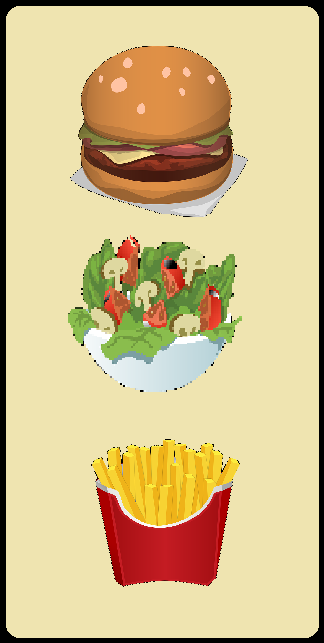
\includegraphics[width=0.2\textwidth]{images/menü_TEMP.png}
                }
        Stell dir vor du gehst in ein Restaurant und du liest folgende Aussage auf der
        Speisekarte: 
        
        \statement{Das Menü enthält einen Burger und Salat oder Pommes}
         
         Wie ist das gemeint? Würde man das Menü bestellen, bekommt man dann einen Burger und darf sich zwischen Salat und Pommes entscheiden oder müsste man sich zwischen Pommes und der Kombination aus Burger und Salat entscheiden? Die deutsche Sprache ist hier uneindeutig und man müsste bei der Bedienung nachfragen.
         
        \end{example}
        Die mathematische Schreibweise für Aussagen wird dieses Problem der Uneindeutigkeit beheben.
    \item Aussagen, die in deutsche Sprache formuliert sind, sind schwer zu lesen und unübersichtlich.
    \begin{example}{}
        Eine Aussage aus dem ersten Beispiel lautete: \statement{Der Zaubertrank ist giftig und ich trinke den Zaubertrank}. Wir werden später sehen, dass eine Formalisierung dieser Aussage wie folgt lautet:
        \[ G \land T\]
        Ohne wissen zu müssen, was diese Symbole bedeuten, sieht man doch, dass diese Formalisierung übersichtlicher ist als die ursprüngliche Aussage. Außerdem kann man diese formalisierte Aussage viel schneller aufschreiben, als die ursprüngliche Aussage. Man spart sich also eine Menge an Schreibarbeit.
    \end{example}
\end{enumerate}

Es ist also hilfreich Aussagen zu formalisieren. Im nächsten Beispiel zeigen wir jetzt beispielhaft, wie wir eine Aussage formalisieren.
\todo{Die Bilder in der letzten Zeile besser positionieren, generell schöner das 'wurde formalisiert zu' in der letzten Zeile darstellen}
\begin{example}{}
    Wir wollen schrittweise die Aussage \statement{Das Menü enthält einen Burger und Salat oder Pommes} formalisieren. 
    \\ \\
    Wir haben bereits in einem vorherigen Beispiel festgestellt, dass der Inhalt dieser Aussage nicht eindeutig ist. Um dieses Problem zu beheben, fügen wir Klammern in die Aussage ein.
    
    \textbf{1. Klammerung:} Wir möchten, dass die Aussage so interpretiert wird, dass das Menü immer aus einem Burger besteht und man sich zwischen Pommes und Salat entscheiden muss. Um das kenntlich zu machen, klammern wir \statement{Salat oder Pommes} ein. Wir erhalten dann: \statement{Das Menü enthält einen Burger und (Salat oder Pommes)}
    \\ \\
    Stell dir vor du möchtest diese Aussage jetzt für verschiedene Rechnungen verwenden. Dann wäre es ziemlich lästig immer diese ganze Aussage aufzuschreiben. Auch das Lesen der Aussage ist anstrengend, da wir immer einen ganzen Satz lesen müssen. Um uns das Leben einfacher zu machen, kürzen wir Unteraussagen durch Symbole ab.
    
    \textbf{2. Unteraussagen durch Symbole ersetzen}: Die Unteraussagen in unserem Beispiel sind:
        \begin{itemize}
            \item \statement{Das Menü enthält einen Burger}
            \item \statement{\textcolor{gray}{Das Menü enthält} Salat} (Kommt nur sinngemäß vor)
            \item \statement{\textcolor{gray}{Das Menü enthält} Pommes} (Kommt nur sinngemäß vor)
        \end{itemize}
    Jede dieser Unteraussagen ersetzen wir jetzt durch ein Symbol, was dann stellvertretend für diese Unteraussage stehen soll. Um sich besser merken zu können für welche Unteraussage ein Symbol steht, ist es sinnvoll das Symbol so zu wählen, dass es irgendwas mit der Unteraussage zu tun hat. Es bietet sich daher an die Unteraussage \statement{Das Menü enthält einen Burger} mit einem Burgersymbol abzukürzen. Wir verwenden folgende Abkürzungen:
    \[\underbrace{\statement{Das Menü enthält einen Burger}}_{\burgerIcn}\statement{~und~}\Bigl(\underbrace{\statement{ Salat}}_{\saladIcn}\statement{~oder~}\underbrace{\statement{Pommes}}_{\friesIcn}\ \ \Bigr)\]
    Wenn wir die Aussage jetzt nur mit den neuen Symbolen aufschreiben, sieht diese nun wie folgt aus:
   \[\burgerIcn \statement{ und } \Bigl(\saladIcn \statement{ oder } \friesIcn\Bigr)\]
    
    Wir sind nun fast fertig mit der Formalisierung. Das Einzige, was noch stört, sind die Konnektoren. Um uns also noch mehr Schreibarbeit zu sparen, ersetzen wir auch diese durch Symbole. Im Gegensatz zu den Unteraussagen, ist aber eindeutig festgeschrieben, welche Konnektoren durch welche Symbole ersetzt werden. 
    
    \textbf{3. Konnektoren durch Symbole ersetzen:} Jedem Konnektor ist ein eindeutiges logisches Zeichen zugeordnet.
    Das Zeichen für \statement{und} ist $\land$ und das Zeichen für \statement{oder} ist $\lor$. Ersetzen wir \statement{und, oder} in der Aussage durch die entsprechenden logischen Symbole, dann erhalten wir:
   
    \[\burgerIcn \land \Bigl( \saladIcn \lor \friesIcn \Bigr)\]
    
    Damit haben wir die ursprüngliche Aussage formalisiert. Um die bessere Lesbarkeit deutlich zu machen, stellen wir einmal die ursprüngliche Aussage neben die formalisierte Aussage:
    \[\begin{array}{c}
        \statement{Das Menü enthält einen Burger und Salat oder Pommes}\\
        \rightsquigarrow\textrm{Wurde formalisiert zu: }\burgerIcn \land \Bigl( \saladIcn \lor \friesIcn \Bigr)
    \end{array}\]
\end{example}

\vspace{30pt}
Wir verallgemeinern jetzt das Vorgehen, mit der wir die Aussage aus dem letzten Beispiel formalisiert haben.
Wenn wir eine beliebige Aussage formalisieren wollen, dann gehen wir wie folgt vor.

\begin{enumerate}
    \item \textbf{Klammerung}: Wir setzen Klammern in der Aussage, um kenntlich zu machen welche Unteraussagen welcher Konnektor miteinander verknüpft.
    \item \textbf{Unteraussagen durch Symbole ersetzen}: Um Schreibarbeit zu sparen, ersetzen wir jede Unteraussage durch ein frei wählbares Symbol. Bestenfalls repräsentieren die eingeführten Symbole den Inhalt der Aussagen, die sie ersetzt haben.
    \item \textbf{Konnektoren durch Symbole ersetzen}: Damit wir noch mehr Schreibarbeit sparen können, führen wir noch weitere Ersetzungen durch. Wir ersetzen dabei jeden Konnektor durch ein fest vorgeschriebenes Symbol. Zum Beispiel ist das Symbol zu \statement{und}, $\land$ und zu \statement{oder}, $\lor$. 
\end{enumerate}

Um den 3. Schritt immer durchführen zu können, muss man sich einmal merken, welches Symbol zu welchem Konnektor gehört. Die zugehörigen Symbole für die Konnektoren \statement{und} und \statement{oder} kennen wir schon. Wir haben aber noch weitere Konnektoren neben diesen beiden kennengelernt. Die nächste Definition zeigt, welche Symbole für welchen Konnektor stehen.

\begin{definition}{}
Die folgende Tabelle definiert welche Konnektoren durch welches Symbol repräsentiert werden.
\begin{center}
\begin{tabular}{cc}\toprule
                Wort/-kombination & Symbol\\\midrule
               und &  $\land$\\
                oder&  $\lor$ \\
                nicht & $\lnot$ \\
                 wenn, dann& $\implies$\\
                genau dann, wenn&  $\iff$ \\
                \bottomrule
\end{tabular}
\end{center}


\end{definition}{}

\todo{Irgendwie Tabelle schöner machen / 3. Beispiel das Negationszeichen näher ans bild}
\begin{example}{}
    Wir zeigen nun noch einmal Aussagen in natürlicher Sprache und eine mögliche Formalisierung dieser. Die Formalisierungen hier sind nicht die einzige Möglichkeit die jeweilige Aussage zu formalisieren. Man hätte ja auch andere Symbole wählen können.
    \begin{center}
    \begin{tabularx}{.8\linewidth}{@{}>{\collectcell\statement}X<{\endcollectcell}@{\hspace{1cm}}r@{}c@{}l@{}}
        \toprule
        \multicolumn{1}{c}{\large Aussage} &  \multicolumn{3}{c}{\large Formalisierung}\\
        \midrule
        Der Trank verleiht Superkräfte \textbf{und} ich trinke den Trank. &
        \superPwrIcn&$\land$&\drinkIcn \\
        Ich trinke den Trank \textbf{oder} ich trinke den Trank \textbf{nicht}. & \drinkIcn&$\lor$& ($\lnot\drinkIcn$)\\
        \textbf{Wenn} der Trank \textbf{nicht} giftig ist, \textbf{dann} trinke ich ihn. & ($\lnot$\poisonIcn)&$\implies$& $\drinkIcn$\\
        Ich trinke den Trank \textbf{genau dann, wenn} er Superkräfte verleiht. & \drinkIcn&$\iff$& \superPwrIcn\\
        \bottomrule
    \end{tabularx}
    \end{center}
\end{example}

Auf dem Papier haben wir nicht die Zeit (und nicht unbedingt die Fähigkeiten), einen Burger, Salat oder Pommes zu malen, um eine Aussage repräsentieren. Es bietet sich dann an, Aussagen einfach mit einem einzelnen Buchstaben abzukürzen. 
 
 \begin{example}{}
 Wir wollen nochmal einmal die Aussage \statement{Das Menü enthält einen Burger und Salat oder Pommes} formalisieren. Wir kürzen die Unteraussagen aber diesmal mit einzelnen Buchstaben ab. Wir verwenden folgende Abkürzungen:
     \[\underbrace{\statement{Das Menü enthält einen Burger}}_{B}\statement{~und~}\Bigl(\underbrace{\statement{ Salat}}_{S}\statement{~oder~}\underbrace{\statement{Pommes}}_{P}\Bigr)\]
Ersetzen wir jetzt die Unteraussagen durch die gerade gewählten Symbole und ersetzen wir noch die Konnektoren durch die entsprechenden Konnektoren, erhalten wir als formalisierte Aussage:
    \[B \land (S \lor P)\]
 \end{example}

\begin{nutshell}

   Aussagen können miteinander zu neuen Aussagen kombiniert werden. Wörter oder Wortkombinationen, die Aussagen zu einer neuen Aussage verknüpfen, nennen wir \textbf{Konnektoren}.
   
   Aussagen, die Teil einer Aussage, nennen wir \textbf{Unteraussagen}.\bigskip
   
   Wenn wir eine Aussage (in deutscher Sprache vorliegend) formalisieren wollen, dann gehen wir wie folgt vor:
   \begin{enumerate}
       \item Klammern setzen, um zu kennzeichnen, welche Unteraussagen die Konnektoren verknüpfen.
       \item Unteraussagen durch frei wählbare Symbole ersetzen. Es bietet sich an als Symbol einen einzelnen Buchstaben zu wählen.
       \item Konnektoren durch fest vorgeschriebene Symbole ersetzen.
   \end{enumerate}
   
    Die folgende Tabelle zeigt durch welche Symbole die Konnektoren in der Formalisierung ersetzt werden müssen.
    
   \begin{center}
       \begin{tabular}{cc}\toprule
            Wort/-kombination & Symbol\\\midrule
            und &  $\land$\\
            oder&  $\lor$\\
            nicht & $\lnot$\\
            wenn, dann& $\implies$\\
            genau dann, wenn&  $\iff$\\\bottomrule
        \end{tabular}
    \end{center}
\end{nutshell}
    
\end{document}